\begin{myex}
 Le tableau suivant donne, dans une population féminine, la moyenne de la tension artérielle en fonction de l'âge :\\
	
		
	\vspace*{-0.5cm}

	\begin{center}
			{\footnotesize  \begin{tabular}{|@{\ }l@{\ }|@{\ }c@{\ }|@{\ }c@{\ }|@{\ }c@{\ }|@{\ }c@{\ }|@{\ }c@{\ }|@{\ }c@{\ }|}
					\hline
					\^Age en années : $x_i$  & 36         & 42         & 48 & 54         & 60         & 66         \\ \hline
					Tension maximale : $y_i$ & \num{11.8} & \num{13.2} & 14 & \num{14.4} & \num{15.5} & \num{15.1} \\ \hline
				\end{tabular}}
	\end{center}
	


	\begin{itemize}
		\item La moyenne des abscisses est : $\bar{x} = 51$;
		\item La moyenne des ordonnées est : $\bar{y} = 14$
		\item Les coordonnées du point moyen G sont donc : $(51 ; 14)$.\\
	\end{itemize}
	
	\vspace*{-0.7cm}
			
	\begin{center}
		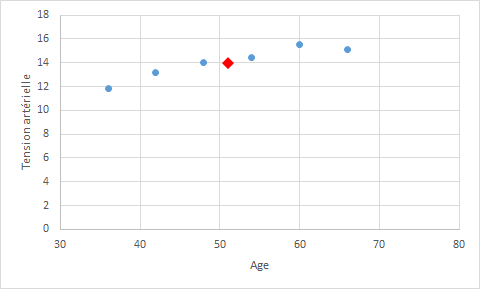
\includegraphics[scale=0.7]{./img/ex1}
	\end{center}


\end{myex}